The purpose of the VRGP is to provide a standardized way of communication for vessels and Maritime Operating Centres (MOC) on the shore. Most importantly, VRGP includes streaming live data from the vessel to the shore and, based on this data, sending guidance messages from the shore to the vessel. This system, a VRGP implementation for the Åboat and, therefore, a maritime system, serves as a proof of concept of the protocol specification and standardizes the external communication of the Åboat.
\\\\
The VRGP implementation will provide the Åboat with the functionality described in the protocol specification, an interface for communication with a MOC. This includes initiating and creating a connection with a MOC, streaming on-board information upon request, terminating a connection, sending notification about abnormal situations on board and receiving guidance from the MOC. The VRGP implementation will be integrated into the existing Åboat architecture and connect with its user interface.
\\\\
The implementation can also be used as a starting point for other implementations. Parts of it will be reusable and the core implementation may even be an independent component to be used by other vessels than the Åboat.

\section{Functional Requirements}\label{sec:func-requirements}

\begin{figure}[ht]
	\centering
	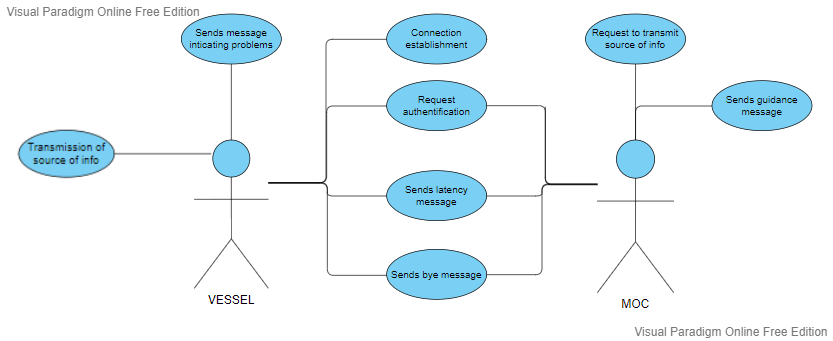
\includegraphics[width=\linewidth]{uml/use-case-diagram}
	\caption{Use case diagram}
	\label{fig:use-case-diagram}
\end{figure}

\subsection{Initiate Connection}

\subsection{Information Streams}

\subsection{Terminate Connection}

\subsection{Authentication}

\subsection{Messages about problems on board}

\subsection{Latency}

\subsection{Clock synchronisation}

\subsection{Guidance}

\section{User Interface Requirements}\label{sec:ui-requirements}

\section{Non-functional Requirements}\label{sec:non-func-requirements}

\subsection{Deliverable}

\subsection{Security}

\subsection{Availability}
